\documentclass[letterpaper]{article}
\usepackage{amssymb}
\usepackage{fullpage}
\usepackage{changepage}
\usepackage{amsmath}
\usepackage{epsfig,float,alltt}
\usepackage{psfrag,xr}
\usepackage[T1]{fontenc}
\usepackage{url}
\usepackage{pdfpages}
\usepackage{epstopdf}
\usepackage[framed,numbered,autolinebreaks,useliterate]{mcode}

%\includepdfset{pagecommand=\thispagestyle{fancy}}
\author{Yi Yang}
\title{SEA Project Report 2}

\begin{document}
\date{09/26/2016}
\maketitle

\newcommand{\trace}{\mathrm{trace}}
\newcommand{\real}{\mathbb R}  % real numbers  {I\!\!R}
\newcommand{\nat}{\mathbb N}   % Natural numbers {I\!\!N}
\newcommand{\cp}{\mathbb C}    % complex numbers  {I\!\!\!\!C}
\newcommand{\ds}{\displaystyle}
\newcommand{\mf}[2]{\frac{\ds #1}{\ds #2}}
\newcommand{\spanof}[1]{\textrm{span} \{ #1 \}}
\newcommand{\sol}[0]{\textbf{Solution: }}
\newcommand{\pf}[0]{\textbf{Proof:}}
\newcommand{\rme}[0]{\textrm{e}}
\newcommand{\Null}[1]{\textrm{Null}\{#1\}}
\parindent 0pt
%%%%%%%%%%%%%%%%%%%%%%%%%%%%%%%%%%%%%%%%%%%%%%%%%%%%%%%%%%%%%%%%%%%%%%%%%%%%%%%
%report starts here!
%%%%%%%%%%%%%%%%%%%%%%%%%%%%%%%%%%%%%%%%%%%%%%%%%%%%%%%%%%%%%%%%%%%%%%%%%%%%%%
This week, I will use some data acquired from the experiment and compare the theoretical curves with the experimental curves.\\
\section*{Test 1}
For data from $SEA\_Free\_K334\_kp10.mat$, I use the following codes:
\lstinputlisting[firstline=1, lastline=100]{SEA_Free_K334_kp10.m}
The plots for simulation and impedance are shown below:
\begin{figure}[H]
	\centering
	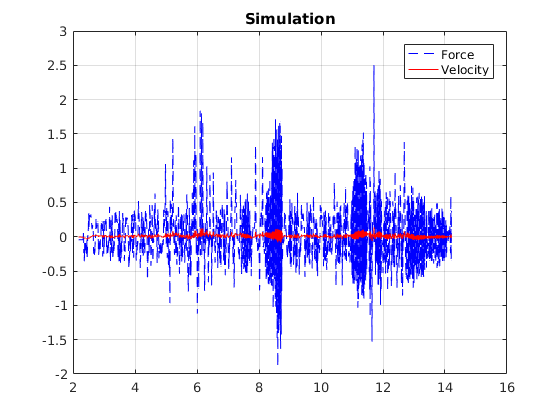
\includegraphics[scale=0.5]{SEA_Free_K334_kp10_sim.png}
	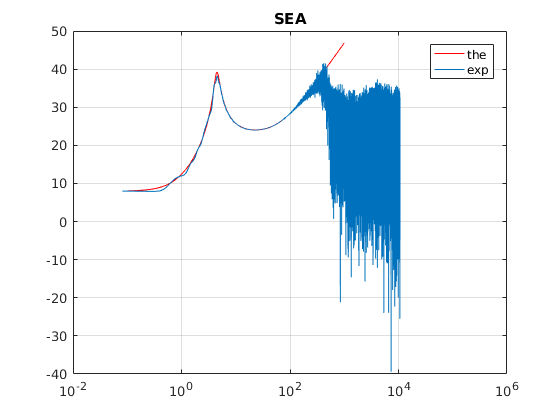
\includegraphics[scale=0.5]{SEA_Free_K334_kp10_impedance.png}
	\caption{Simulation of Linear Matlab Model}
	\label{fig:sim}
\end{figure}

\vspace*{1em}
\textbf{Remark:}
\begin{itemize}
	\item the experiment data I use for the above test experiment is $RevPosB$, and use it to calculate user force $Fuser$
	\item I apply $Fuser$ to the linear matlab model, using $lsim$ function to get the output data $U_o$
	\item The last step is to estimate the transfer function using $Fuser$ and $U_o$.
\end{itemize}

Next, I will estimate transfer function from input and output data sets that are all measured from experiments (real data).
\section*{Test 2}
For admittance device, we use data set with $K_p=-3$ and $K_{ve}=400$. Matlab codes are shown below:
\lstinputlisting[firstline=1, lastline=100]{adm_Kp3_Kev100.m}
\begin{figure}[H]
	\centering
	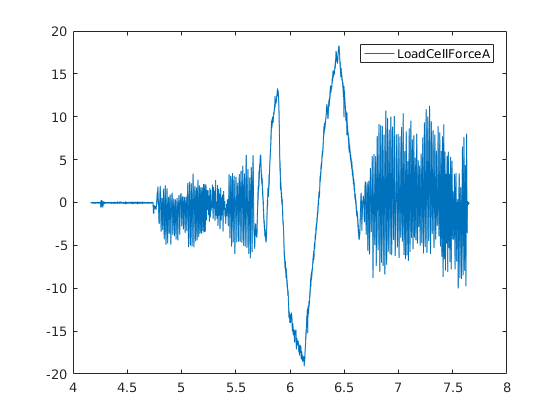
\includegraphics[scale=0.5]{adm_loadcellforceA.png}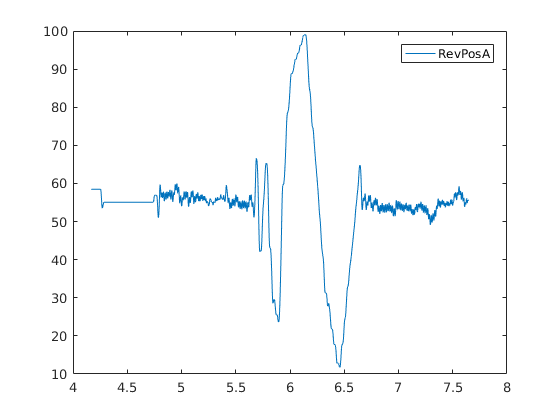
\includegraphics[scale=0.5]{adm_revposA.png}
	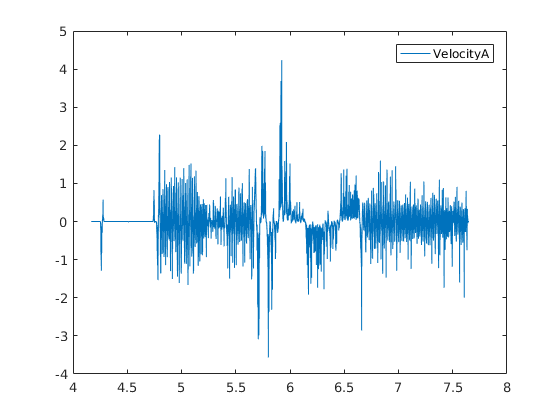
\includegraphics[scale=0.5]{adm_velocityA.png}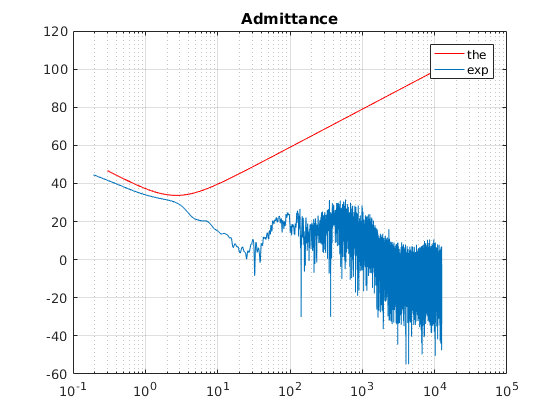
\includegraphics[scale=0.5]{adm_impedance.png}
	\caption{LoadCellForceA, RevPosA, Actual VelocityA, Driving Point Impedance}
\end{figure}

\section*{Test 3}
For SEA device, we use data sets with $K_p=-3$, $K_{ve}=400$ and $K_{spring}=1200$. Matlab codes shown below:
\lstinputlisting[firstline=1, lastline=100]{sea_Kp3_Kev100.m}
\begin{figure}[H]
	\centering
	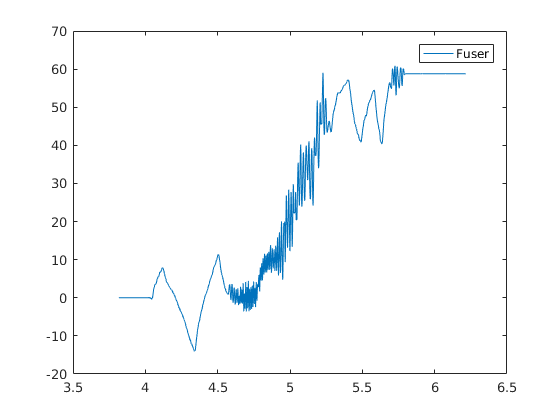
\includegraphics[scale=0.5]{sea_fuser.png}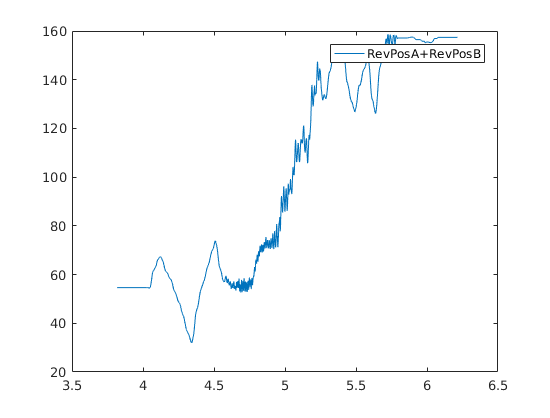
\includegraphics[scale=0.5]{sea_revposA_B.png}
	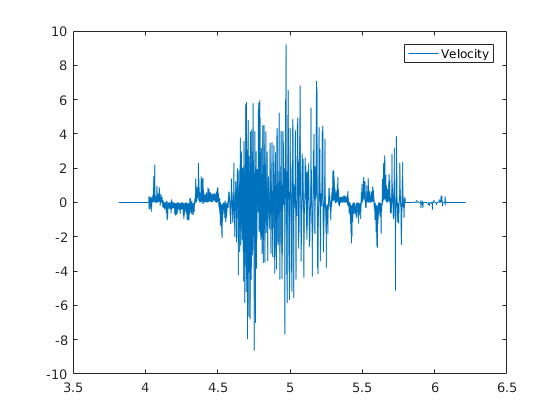
\includegraphics[scale=0.5]{sea_velocity.png}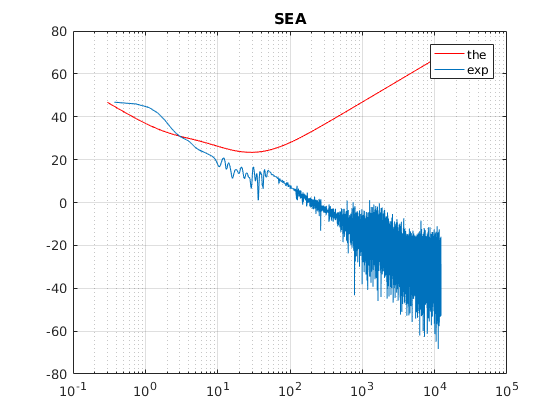
\includegraphics[scale=0.5]{sea_impedance.png}
	\caption{Fuser, Actual Position, Actual Velocity, Driving Point Impedance}
	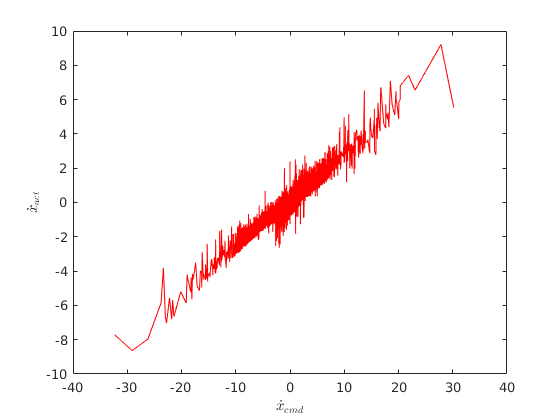
\includegraphics[scale=0.8]{sea_vv.png}
	\caption{Actual Velocity Vs Command Velocity}
\end{figure}
\end{document}